
\chapter{Voyaging on H\=ok\=ule\kern.05em`\kern.05em\relax a}


\begin{quotation}
``When we voyage, and I mean voyage anywhere, not just in canoes, but in our minds, new doors of knowledge will open, and that's what this voyage is all about\dots it's about taking on a challenge to learn. If we inspire even one of our children to do the same, then we will have succeeded.''\\
--Nainoa Thompson, September 20, 1999, the day of departure for the challenge of navigating from Mangareva to Rapa Nui, the remotest, most difficult island to navigate to in Polynesia.
\end{quotation}


\bigskip

In the 1950s and 1960s, historians couldn't agree on how the Polynesian islands --- including the Hawaiian islands --- were settled.  Some historians insisted that Pacific Islanders sailed around the Pacific Ocean, relocating as necessary, and 
 settling  the islands with purpose and planning.   Others insisted that such a navigational and voyaging feat was impossible thousands of years ago, before European sailors would leave the sight of land and sail into the open ocean.  These historians believed that the Polynesian canoes were caught up in storms, tossed and turned, and eventually washed up on the shores of faraway isles.
 
 
 \bigskip
 
 
 \begin{thinkpair*}
 Talk about these questions with a partner:
 \begin{itemize}
 \item 
 How could such a debate ever be settled one way or the other, given that we can't go back in time to find out what happened?\\
 
 \item
 What kinds of evidence would support the idea of ``intentional voyages''?  What kinds of evidence would support the idea of ``accidental drift''?  \\
 
 \item
 What do you already know about how this debate was eventually settled?
 \end{itemize}
 \end{thinkpair*}


\newpage

\section{H\=ok\=ule\kern.05em`\kern.05em\relax a}

The Polynesian Voyaging Society (PVS) was founded in 1973 for scientific inquiry into the history and heritage of \Hawaii: How did the Polynesians discover and settle these islands?
 How did they navigate without instruments, guiding themselves across ocean distances of 2500 miles? 
 
 In 1973--1975, PVS built a replica of an ancient double-hulled voyaging canoe to conduct an experimental voyage from \Hawaii\ to Tahiti. The canoe was designed by founder Herb Kawainui K\=ane and named \Hokulea, Star of Gladness.
 
 
  On March 8th, 1975, \Hokulea\ was launched.  Mau Piailug, a master navigator from the island of Satawal in Micronesia, navigated her to Tahiti using traditional navigation techniques (no modern instruments at all).


 \bigskip
 
 \begin{thinkpair*}
 Brainstorm with a partner:
 \begin{itemize}
 \item
What are some \emph{mathematical} questions you can ask about voyaging on \Hokulea?\\

\item
What kinds of problems (especially mathematics problems) did the crew have to solve before setting off on the voyage to Tahiti?\\

\item
What are you curious about, with respect to voyaging on \Hokulea?\\
\end{itemize}
 \end{thinkpair*}

\bigskip
\bigskip

When you teach elementary school, you will mostly likely be teaching all subjects to your students.  One thing you should think about as a teacher: How can you connect the different subjects together?  How can you see mathematics in other fields of study, and how can you draw out that mathematical content?

In this chapter, you'll explore just a tiny bit of the mathematics involved in voyaging on a traditional canoe.  You will apply your knowledge of geometry to create scale drawings and make a star compass.  And you'll use you knowledge of operations and algebraic thinking to plan the supplies for the voyage.  The focus here is on applying your mathematical knowledge to a new situation.

\newpage

One of the first things to know about \Hokulea\ is what she looks like.   This picture and drawing of \Hokulea\ come from the PVS website: \url{http://hokulea.org}.

\bigskip

\begin{center}
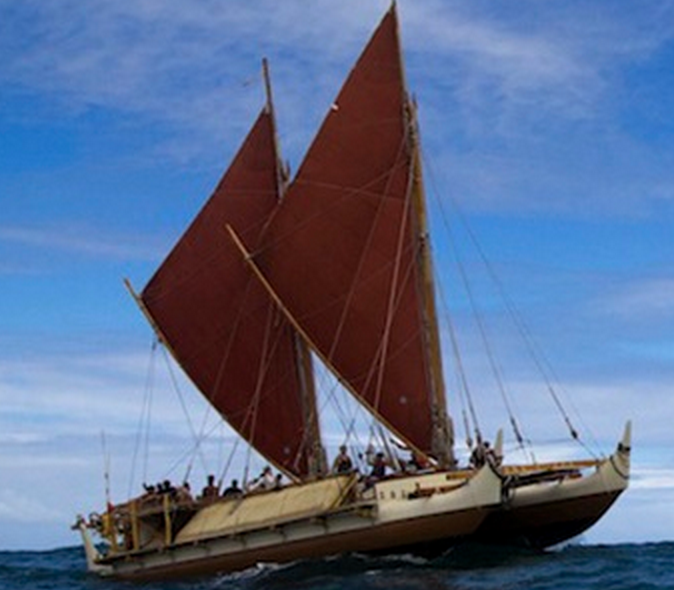
\includegraphics[height=8cm]{hokulea}
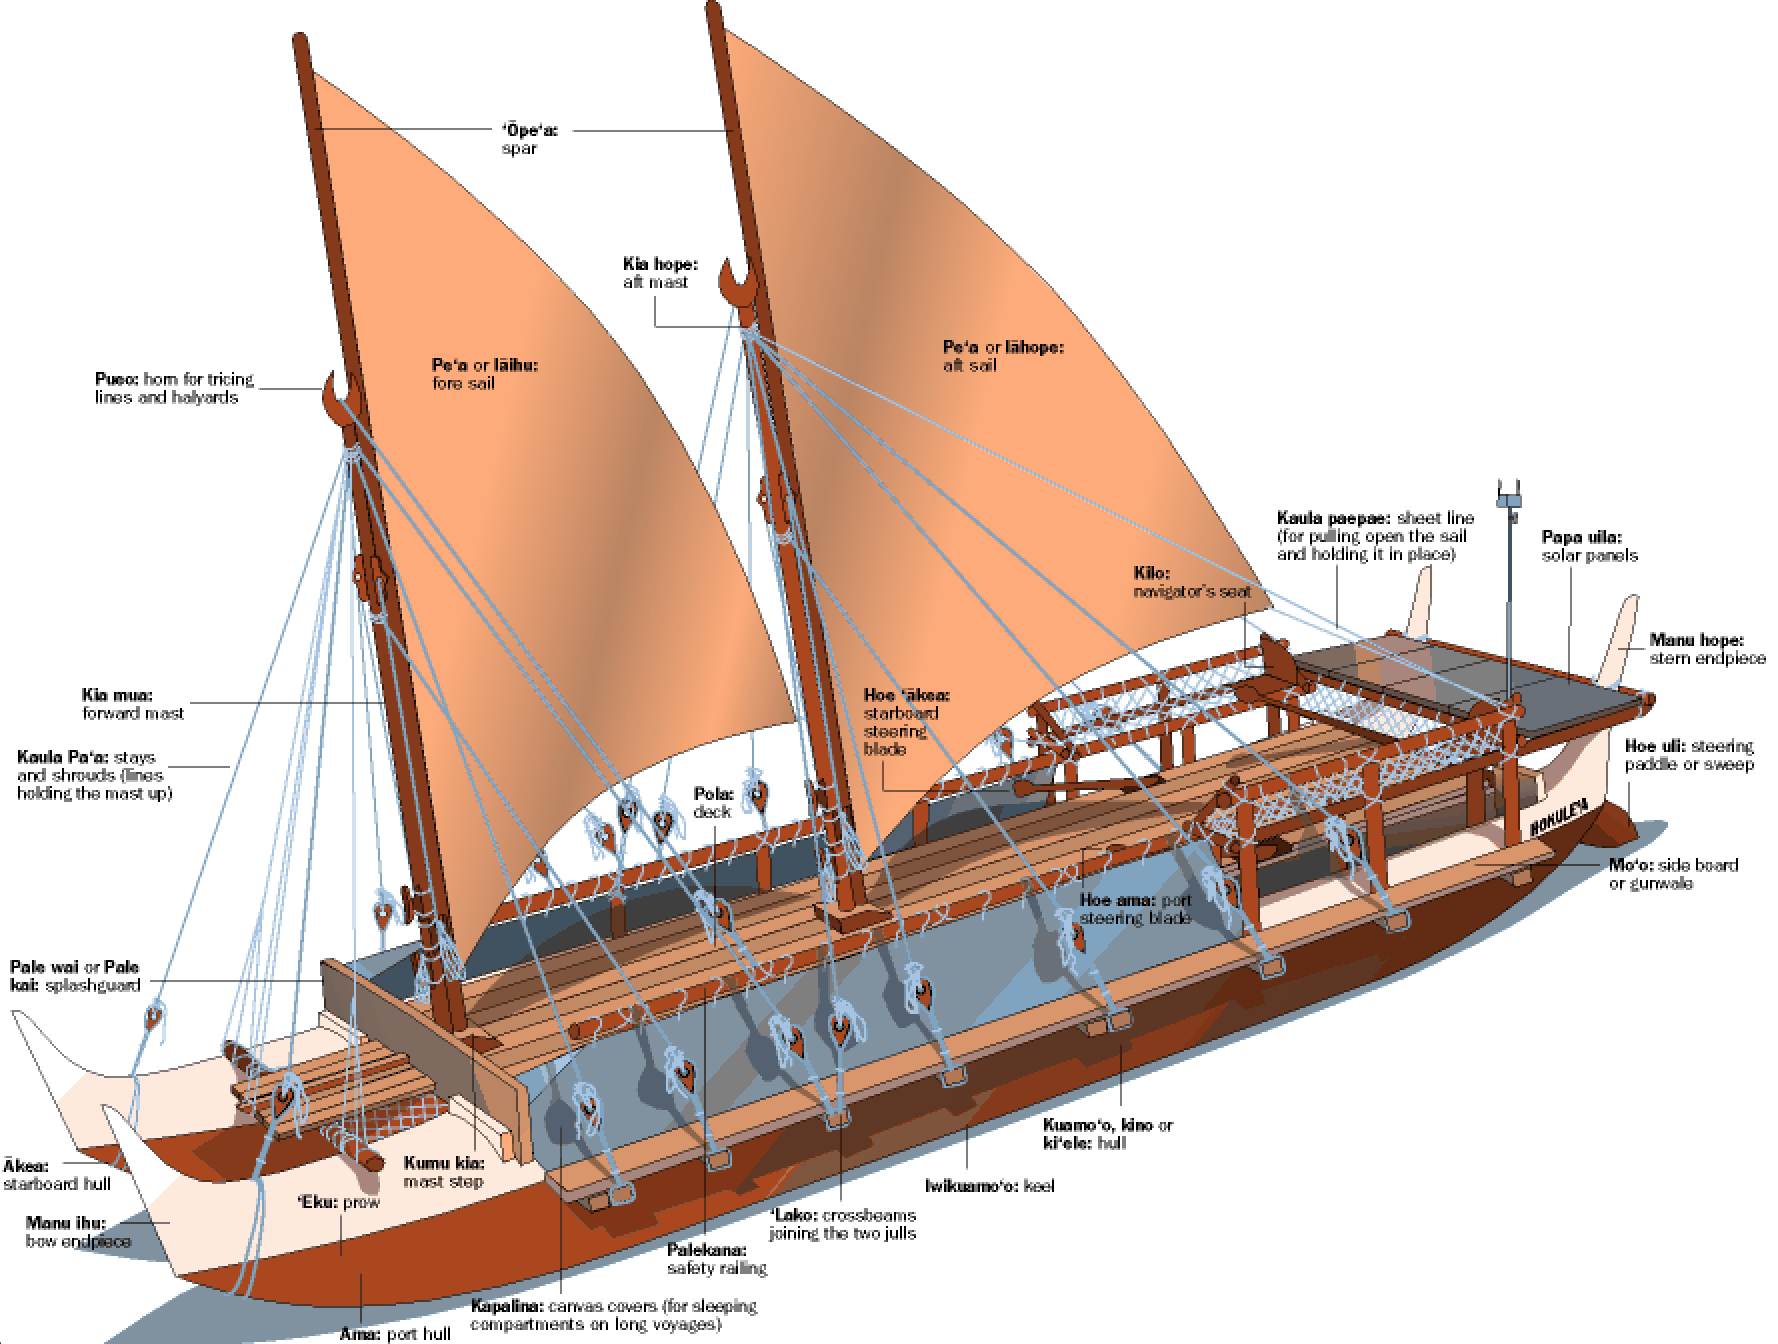
\includegraphics[height=10cm]{hokulea_drawing}
\label{hokuleapics}
\end{center}

\bigskip

\begin{problem}\label{scaledraw}
Here's  some information about the dimensions of \Hokulea.  Your job is to draw a  good scale model of the canoe, like a floorplan.  Imagine you are above the canoe looking down at it.  Draw a scale model of what you would see.  Do not include the sails or any details; you are aiming to convey the overall shape in a scale drawing.  You will use this scale drawing several times in the rest of this unit, so be sure to do a good job and keep it somewhere that you can find it later.\\

\begin{itemize}
\item
\Hokulea\ is 62 feet 4 inches long.  (This is ``LOA'' or ``length overall'' in navigation terms.  It means the maximum length measured parallel to the waterline.)\\

\item
\Hokulea\ is 17 feet 6 inches wide.  (This is ``at beam'' meaning at the widest point.)\\

\item
You can see from the picture that \Hokulea\ has two hulls, connected by a rectangular deck.   The deck is about 40 feet long and 10 feet wide.\\

\end{itemize}

\noindent
 {\bf Note:}  You don't have all the information you need!  So you either need to find out the missing information or make some reasonable estimates based on what you do know.\\



\end{problem}


\bigskip

\begin{problem}
Crew for a voyage is usually 12--16 people.  During mealtimes, the whole crew is on the deck together.  About how much space does each person get when they're all together on the deck?

\end{problem}

\newpage

\section{Worldwide Voyage}
To prepare for the next activity:
\begin{itemize}

\item
Read this description of the daily life on \Hokulea: \url{http://pvs.kcc.hawaii.edu/ike/canoe_living/daily_life.html}.  \\

\item
Watch the video about the  Worldwide Voyage: \url{http://vimeo.com/51118047}.\\
\end{itemize}


From the webpage above, you learned:
\begin{quote}
``The quartermaster is responsible for provisioning the canoe --- loading food, water and all needed supplies, and for maintaining \Hokulea's inventory. While this is not an on board job, it is critical to the safe and efficient sailing of the canoe.''
\end{quote}


\begin{problem}
Imagine that you are part of the crew for the  Worldwide Voyage, and you are going to help the quartermaster and the captain with provisioning the canoe for one leg of the voyage.  You need to write a preliminary report for the quartermaster, documenting:
\begin{itemize}
\item
Which leg of the trip are you focused on?  (See the map below.)\\


\item
How long will that leg of the trip take?  Explain how you figured that out.\\

\item
How much food and water will you need for the voyage?  Explain how you figured that out.\\
\end{itemize}
\end{problem}

The rest of this section contains pointers to information that may or may not be helpful to you as you make your plans.  Your job is to do the relevant research and then write your report.  You should include enough detail about how you came to your conclusions that the quartermaster can understand your reasoning.  Note: 
during \Hokulea's voyage, you can track the progress here: \url{http://www.hokulea.com/track-the-voyage/}.  



\subsection*{Pick a leg of the route}
Here's a picture of the route planned for the Worldwide Voyage, which you can find at the Worldwide Voyage website \url{http://hokulea.org/world-wide-voyage/}.  Note that on the map, the different colors correspond to different years of the voyage.  A ``leg'' means a dot-to-dot route on the map.




\begin{center}
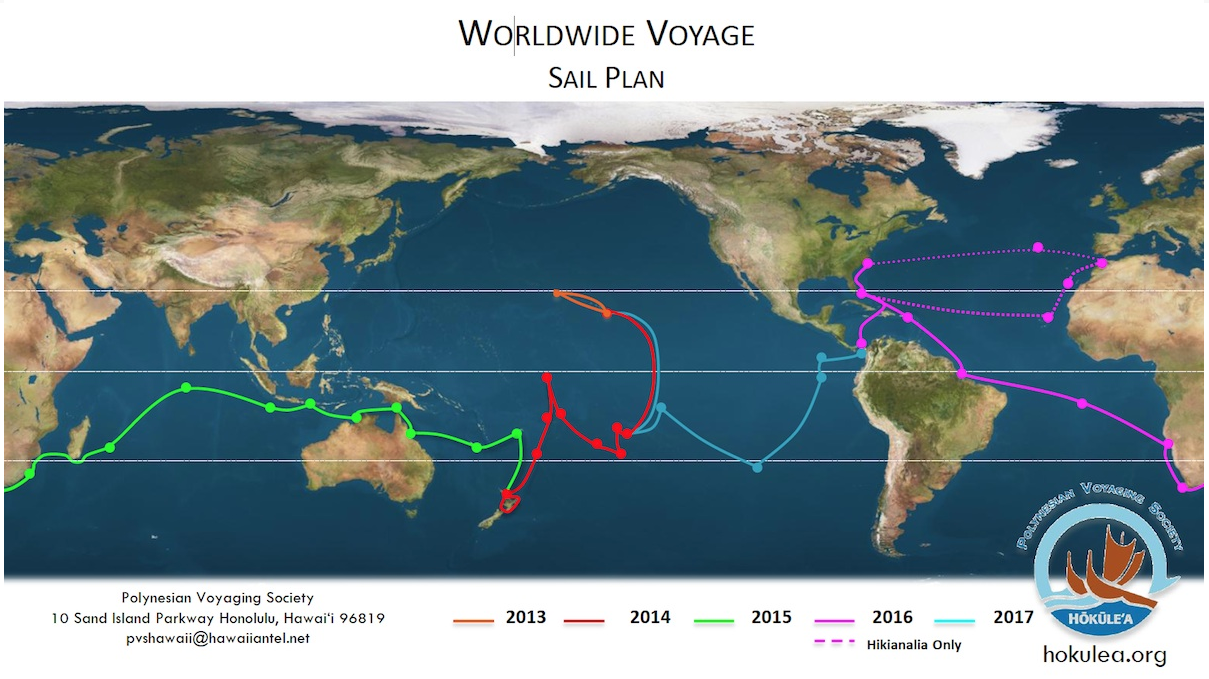
\includegraphics[height=7cm]{wwvroute}
\end{center}


After you pick a leg of the voyage, you'll need to figure out the total distance of that leg.  This tool might help (or you can find another way): \url{http://www.acscdg.com/}.
  Here is some relevant information to help you figure out how long it will take \Hokulea\ to complete that leg:

\begin{itemize}
\item
Fully loaded with the maximum weight,  \Hokulea\ can travel at speeds of 4--6 knots, and even 10--12 knots in strong winds.  (One knot means one nautical mile per hour.)\\

\item
For comparison, the first trip from \Hawaii\ to Tahiti in 1976 took a total of 34 days.  (You probably want to use the tool above to compute the number of nautical miles.) \\

\end{itemize}

\subsection*{Plan the provisions}
Here is some information about provisions.  

\begin{itemize}
\item
Hokulea can carry about 11,000 pounds, including the weight of the crew, provisions, supplies, and personal gear.  \\

\item
The supplies (sails, cooking equipment, safety equipment, communications equipment, etc.) account for about 3,500 pounds. \\

\item
The crew eats three meals per day and each crew member gets  $0.8$ gallons of water per day.\\


\item
For a trip that is expected to take 30 days, the quartermaster plans for 40 days' worth of supplies, in case of bad weather and other delays.\\


\end{itemize}

\newpage





\section{Navigation}
The following is from \url{http://pvs.kcc.hawaii.edu/ike/hookele/modern_wayfinding.html}:
\begin{quote}
``A voyage undertaken using modern wayfinding has three components:

\begin{enumerate}
\item
Design a course strategy, which includes a reference course for reaching the vicinity of one's destination, hopefully upwind, so that the canoe can sail downwind to the destination rather than having to tack into the wind to get there. (Tacking involves sailing back and forth as closely as possible into the wind to make progress against the wind; it�s very arduous and time-consuming, something to be avoided if at all possible, particularly at the end of a long, difficult voyage.)

\item
 During the voyage, holding as closely as possible to the reference course while keeping track of (1) distance and direction traveled; (2) one's position north and south and east and west of the reference course and (3) the distance and direction to the destination.

\item
Finding land after entering the vicinity of the destination, called a target screen or `the box'.''

\end{enumerate}
\end{quote}

So how is the navigation done --- especially component (2) ---  through thousands of miles of open ocean?  You can't see land.  How can you hold closely to the reference course?  How can you keep track of distance and direction traveled?  How can you even know if you're going in the right direction?

By day, the navigators use their deep knowledge of the oceans.  Which way do the winds blow?  Which way do the prevailing currents move?  Clouds in the sky, flotsam in the water,  and animal behaviors can give you great insight into where land might be, and where you are in relation to it.

By night, they use the stars.  In this section, you'll learn just a tiny fraction of what these master navigators know about the stars.


\newpage

\begin{thinkpair*}
Here is a time-lapse picture of the stars in the night sky in \Hawaii.  

\begin{center}
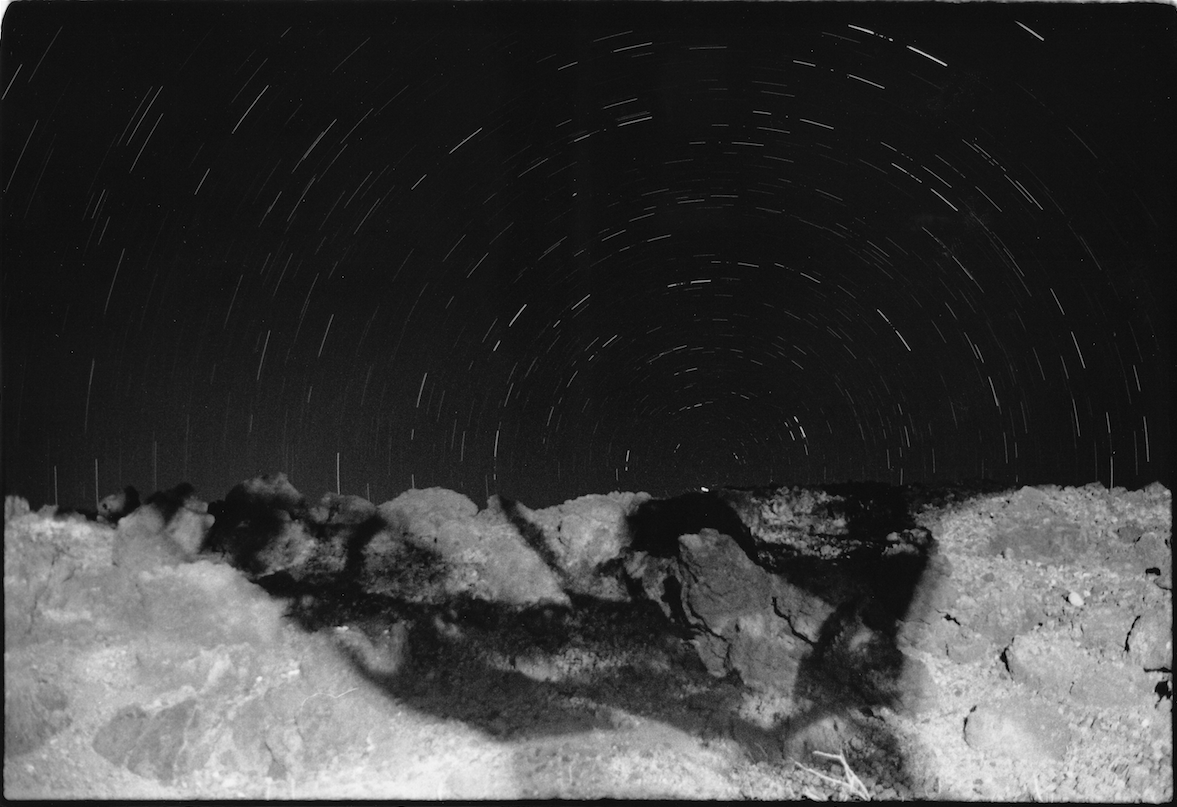
\includegraphics[height=9cm]{stars2}
\label{starpic}

Photography by Ashley Deeks.
\end{center}

\begin{itemize}
\item
Describe what you see happening in this picture. \\
\item
 What can you conclude about how the stars move through the night sky? \\
 \item
  How might that help a navigator find his way?
  \end{itemize}


\end{thinkpair*}




\newpage



\subsection{Star Compass}
A fundamental tool for navigators on \Hokulea\ and other voyaging canoes is a star compass.
Here's a picture of Mau Piailug building a star compass to teach navigation.  

\begin{center}
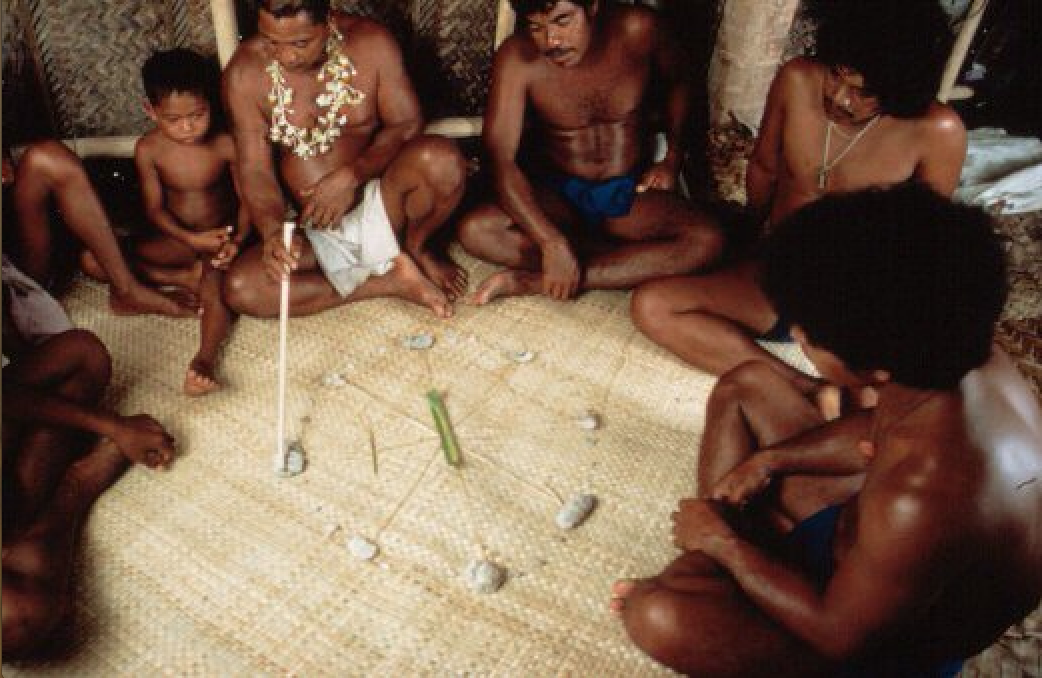
\includegraphics[height=7cm]{MauKids}

Picture from \url{http://pvs.kcc.hawaii.edu/holokai/2007/mau_1_intro.html}.

\end{center}


The object in the center of the circle represents the canoe.  The rocks along the outside represent directional points.  The idea is to imagine the stars rising up from the horizon in the east, traveling through the night sky, and setting past the horizon in the west.  They move like they're on a sphere surrounding the Earth (it's called the \emph{celestial sphere}).

\bigskip

\begin{problem}
Nainoa Thompson developed a star compass with 32 equidistant points around a circle.  (Note this is more points than in Mau's star compass above.)  You will try first to make a rough sketch of Nainoa's star compass based on this information:

\begin{itemize}
\item
Place 32 points around the circle so they are equally spaced.  \\

\item
The arcs between these equidistant points are called ``houses.''  You will label each house with its Hawaiian name.  Start with the four cardinal points:
\begin{description}
\item[North]   `\kern.05em\relax Akau.
\item[South]   Hema.
\item[East]  Hikina.
\item[West]  Komohana.\\
\end{description}

\item
The four quadrants also get names.  (These cover all of the houses in the quadrant, so label them in the appropriate place inside the compass.)
\begin{description}
\item[Ko`\kern.05em\relax olau]  northeast.
\item[Malani]   southeast.
\item[Kona]  southwest.
\item[Ho`\kern.05em\relax olua] northwest.\\
\end{description}



\item
Moving from `\kern.05em\relax Akau to Hikina (clockwise), there are seven houses.  They are labeled in order as you move away from `\kern.05em\relax Akau:
\begin{description}
\item[Haka] ``empty,'' describing the skies  in this house.
\item[N\=a Leo] ``the voices'' of the stars speaking to the navigator.
\item[N\=alani] ``the heavens.''
\item[Manu] ``bird,'' the  Polynesian metaphor for a canoe.
\item[Noio] the Hawaiian tern (a bird)
\item[`\kern.05em\relax\=Aina] ``land.''
\item[L\=a] ``sun,'' which stays in this house most of the year.
\\
\end{description}


\item
The compass has a vertical line of symmetry, so there are the same seven houses in the same order as you move from `\kern.05em\relax Akau to Komohana (counterclockwise).\\ 

\item
The compass also has a horizontal line of symmetry.  Use that fact to label the houses from Hema to Hikina (counterclockwise) and from Hema to Komohana (clockwise).


 
\end{itemize}
\end{problem}

\bigskip
\bigskip


How is the star compass used in navigation?  There are lots of ways.  Here's a (very!) quick overview:

\fellow{I don't know if there's any way to do an animation of this description, but if so it would be cool!}

\begin{itemize}
\item
The canoe is pictured in the middle of the star compass, with all of the houses around. \\
\item
Winds and ocean swells move directly \emph{across} the star compass from north to south or vice versa.  
\begin{itemize}
\item
If the swells are coming from   `\kern.05em\relax\=Aina Ko`\kern.05em\relax olau, they will be heading in the direction  `\kern.05em\relax\=Aina Kona.  (Look at your star compass and trace out this path.)
\item
 If the wind is coming from   N\=alani Malani, it will be heading towards   N\=alani Ho`\kern.05em\relax olua.   (Look at your star compass and trace out this path.)\\
\end{itemize}

\item
Stars stay in their houses, but also in their hemisphere.  Just like the sun, they rise in the east and set in the west; they do not move across the center of the circle. 

\begin{itemize}
\item
 \Hokulea\  rises in   `\kern.05em\relax\=Aina Ko`\kern.05em\relax olau and sets in  `\kern.05em\relax\=Aina Ho`\kern.05em\relax olua.  (Look at your star compass and trace out this path.)
\item
 `\kern.05em\relax A`\kern.05em\relax\=a (Sirius) rises in  L\=a Malanai and sets in  L\=a Kona.\\
\end{itemize}

\end{itemize}

A navigator memorizes the houses of over 200 stars.  At sunrise and sunset (when the sun or the stars are rising), the navigator can use the star compass to  memorize which way the wind is moving and which way the currents are moving.  He can then use that information throughout the day or night to ensure the canoe stays on course.


\bigskip
\bigskip

\begin{thinkpair*}
Look again at the time-lapse picture of the stars. 

\begin{center}
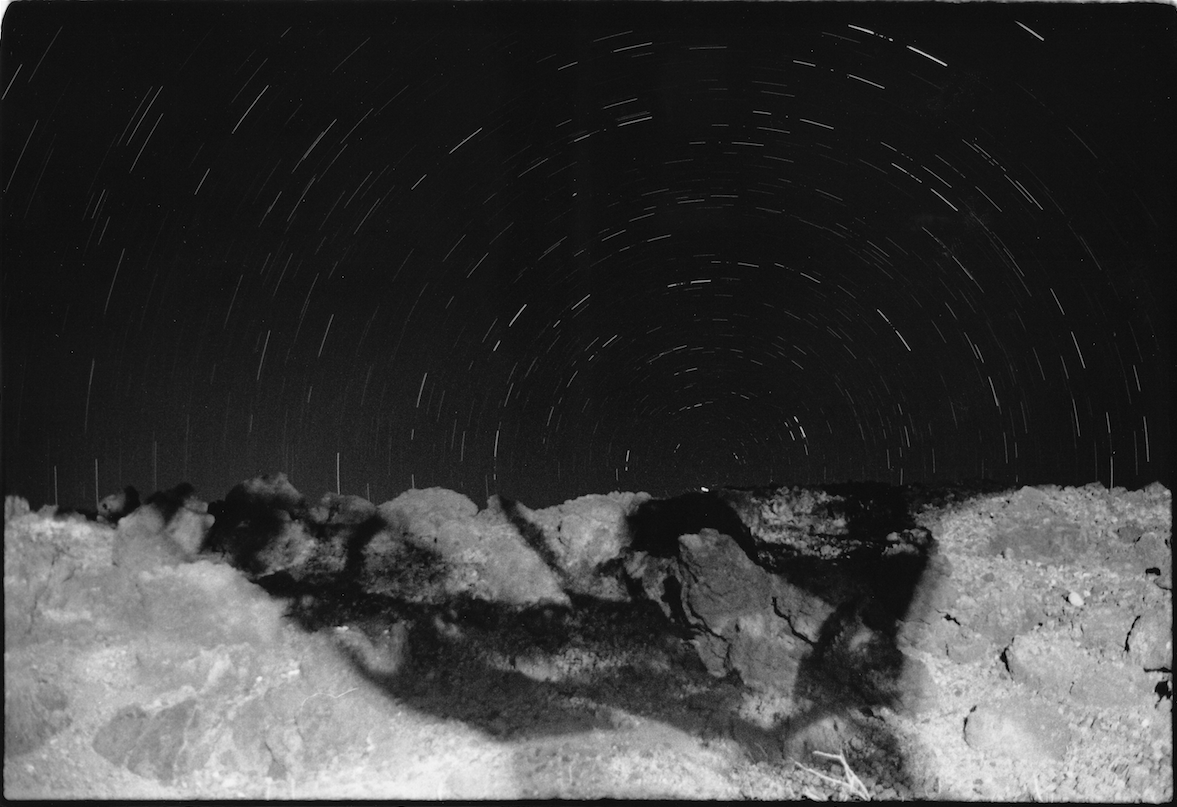
\includegraphics[height=9cm]{stars2}
\label{starpic}

Photography by Ashley Deeks.
\end{center}
\begin{itemize}
\item
 Describe how this shows that stars ``stay in their houses'' and in their hemisphere as they move through the night sky.\\
 \item
The star Ke ali'i o kona i ka lewa (Canopus),  rises in N\=alani Malanai.  Where does it set?
\end{itemize}
\end{thinkpair*}



When teaching navigation while sitting on land, it's perfectly fine to have a rough sketch or model of the star compass.  But if you really have to do the navigation, you need to make a very, very precise star compass.  

Imagine Nainoa Thompson,  who navigated  \Hokulea\ on the final leg of her journey  from \Hawaii\ to Rapa Nui, an island even smaller and lower than Ni\kern.05em\relax ihau.  You have to be within 30 miles of Rapa Nui to see it.  But  a mistake of even one degree   would have led to \Hokulea\ being 60 miles off course.  And if you end up drifting in the open ocean and supplies run out?  Well\dots 


\bigskip

\begin{problem}
Now that you have a rough sketch of the star compass and know what it should look like, your job is to draw one that's as perfect as possible.  That means you want to draw:
\begin{itemize}
\item
A perfect circle (well, as perfect as possible).  What tools can you use to do that?  What tools would ancient Polynesian navigators have had to use?\\

\item
Thirty-two points around the circle that are \emph{exactly} evenly spaced apart.  (What tools would help you?    What tools would ancient Polynesian navigators have had to use?) \\

\item
When you have finished, label your perfectly drawn star compass with the houses.
\end{itemize}

\end{problem}


\bigskip




\bigskip


Of course, a star compass on a piece of paper isn't so useful when you're out on a canoe.  How do you position it properly?  And how do you keep it from getting lost, damaged, or soaking wet?  You paint it on the rails of the canoe, permanently!

Look back at the drawing of \Hokulea\ on page~\pageref{hokuleapics}.  Find the ``kilo'' (navigator's seat) in the rear (aft) of the canoe.  There is actually one navigator's seat on either side of the deck.

\bigskip

\begin{problem}
Go back to the scale drawing of \Hokulea\ that you made in Problem~\ref{scaledraw}.  Add the navigator's seats to your drawing.  You will then add the star compass to the rails as follows:

\begin{itemize}
\item
Start with the seat on the left (port side) of the canoe.  That will be the center of your star compass.  Imagine looking to the right.  You want to see the star compass markings on the rails when you look to the right.  Of course, the \Hokulea\ is not a circular canoe, and the navigator doesn't sit at the center.  So how can you make the markings in the right places?\\

\item
Now repeat that process, using the seat on the right (starboard) side of the canoe.\\

\end{itemize}

\end{problem}

\bigskip


Nainoa Thompson has said: 

\begin{quote}
``Initially, I depended on geometry and analytic mathematics to help me in my quest to navigate the ancient way. However as my ocean time and my time with Mau have grown, I have internalized this knowledge. I rely less on mathematics and come closer and closer to navigating the way the ancients did.''
\end{quote}

\bigskip
\bigskip

Really he is still doing a lot of mathematics; it's just mathematics that he has internalized and is now second nature to him.  The ancient navigators may not have spoken of their navigation techniques in the same modern language we've been using --- compass points and perfect circles and degrees.  But their mathematical understanding was truly astonishing.









